% Recent large language models (LLMs), especially when augmented with reasoning and tool-use capabilities, have achieved strong performance on a range of cognitively demanding tasks, including code editing, mathematical problem solving, and complex information retrieval \citep{swe-bench, hle, omni-olpc}. However, growing evidence suggests that such capabilities do not yet translate into robust, general-purpose autonomy across the full spectrum of human cognitive labor \citep{amodei2024machines, kwa2025measuringaiabilitycomplete, aisi2025limitations}. In particular, prior work shows that superhuman or near-superhuman performance is largely limited to short-horizon or highly structured settings, while performance degrades in tasks requiring long-term planning, persistent goal maintenance, and adaptation to dynamic environments \citep{kwa2025measuringaiabilitycomplete, metr2025measuring}.

% To evaluate LLM-based agents in more realistic settings, prior work has introduced agent-based benchmarks covering web interaction \citep{mialon2023gaiabenchmarkgeneralai, browsecomp, webarenarea, mind2web}, code editing \citep{swe-bench, tbench_2025}, and multimodal understanding \citep{mmmupro, videommmu}. While effective, these benchmarks primarily focus on short-horizon tasks with limited temporal dependencies, limiting their ability to assess sustained interaction with complex, evolving environments. Recent simulation-based benchmarks targeting long-horizon autonomy \citep{nof1, andonlabs2025vendingbench2, backlund2025vendingbenchbenchmarklongtermcoherence} consistently show that even state-of-the-art agents struggle to maintain coherent strategies over extended time spans.

% In this work, we introduce a new benchmark grounded in real-world commercial data and informed by established economic modeling principles. We focus on a supermarket operation scenario, which requires long-term decision-making, continual interaction with a dynamic environment, and the integration of heterogeneous information sources. The benchmark evaluates whether LLM-based agents can autonomously sustain realistic business operations under dynamic, multi-factor conditions.

% Our contributions are summarized as follows:

% \begin{itemize}[leftmargin=*]
% \item We introduce a high-fidelity business simulation environment that models key aspects of real-world retail operations, including inventory management, pricing and sales dynamics, supply-chain control, customer feedback, and external news events. The environment captures realistic operational constraints and temporal dependencies, enabling systematic evaluation of long-horizon agent behavior. We further propose the \textit{Evolving Strategy \& Execution Agent} framework, which outperforms a Reflection-based baseline across all evaluated metrics.

% \item 
% \end{itemize}

Recent large language models (LLMs) achieve strong performance on short-horizon tasks \citep{swe-bench, hle, omni-olpc} but struggle with long-horizon autonomy \citep{amodei2024machines, kwa2025measuringaiabilitycomplete, metr2025measuring}. Existing agent benchmarks focus primarily on short-horizon tasks \citep{mialon2023gaiabenchmarkgeneralai, browsecomp, webarenarea, mind2web}, limiting their ability to evaluate sustained interaction with complex environments.

\begin{figure*}[t]
\begin{center}
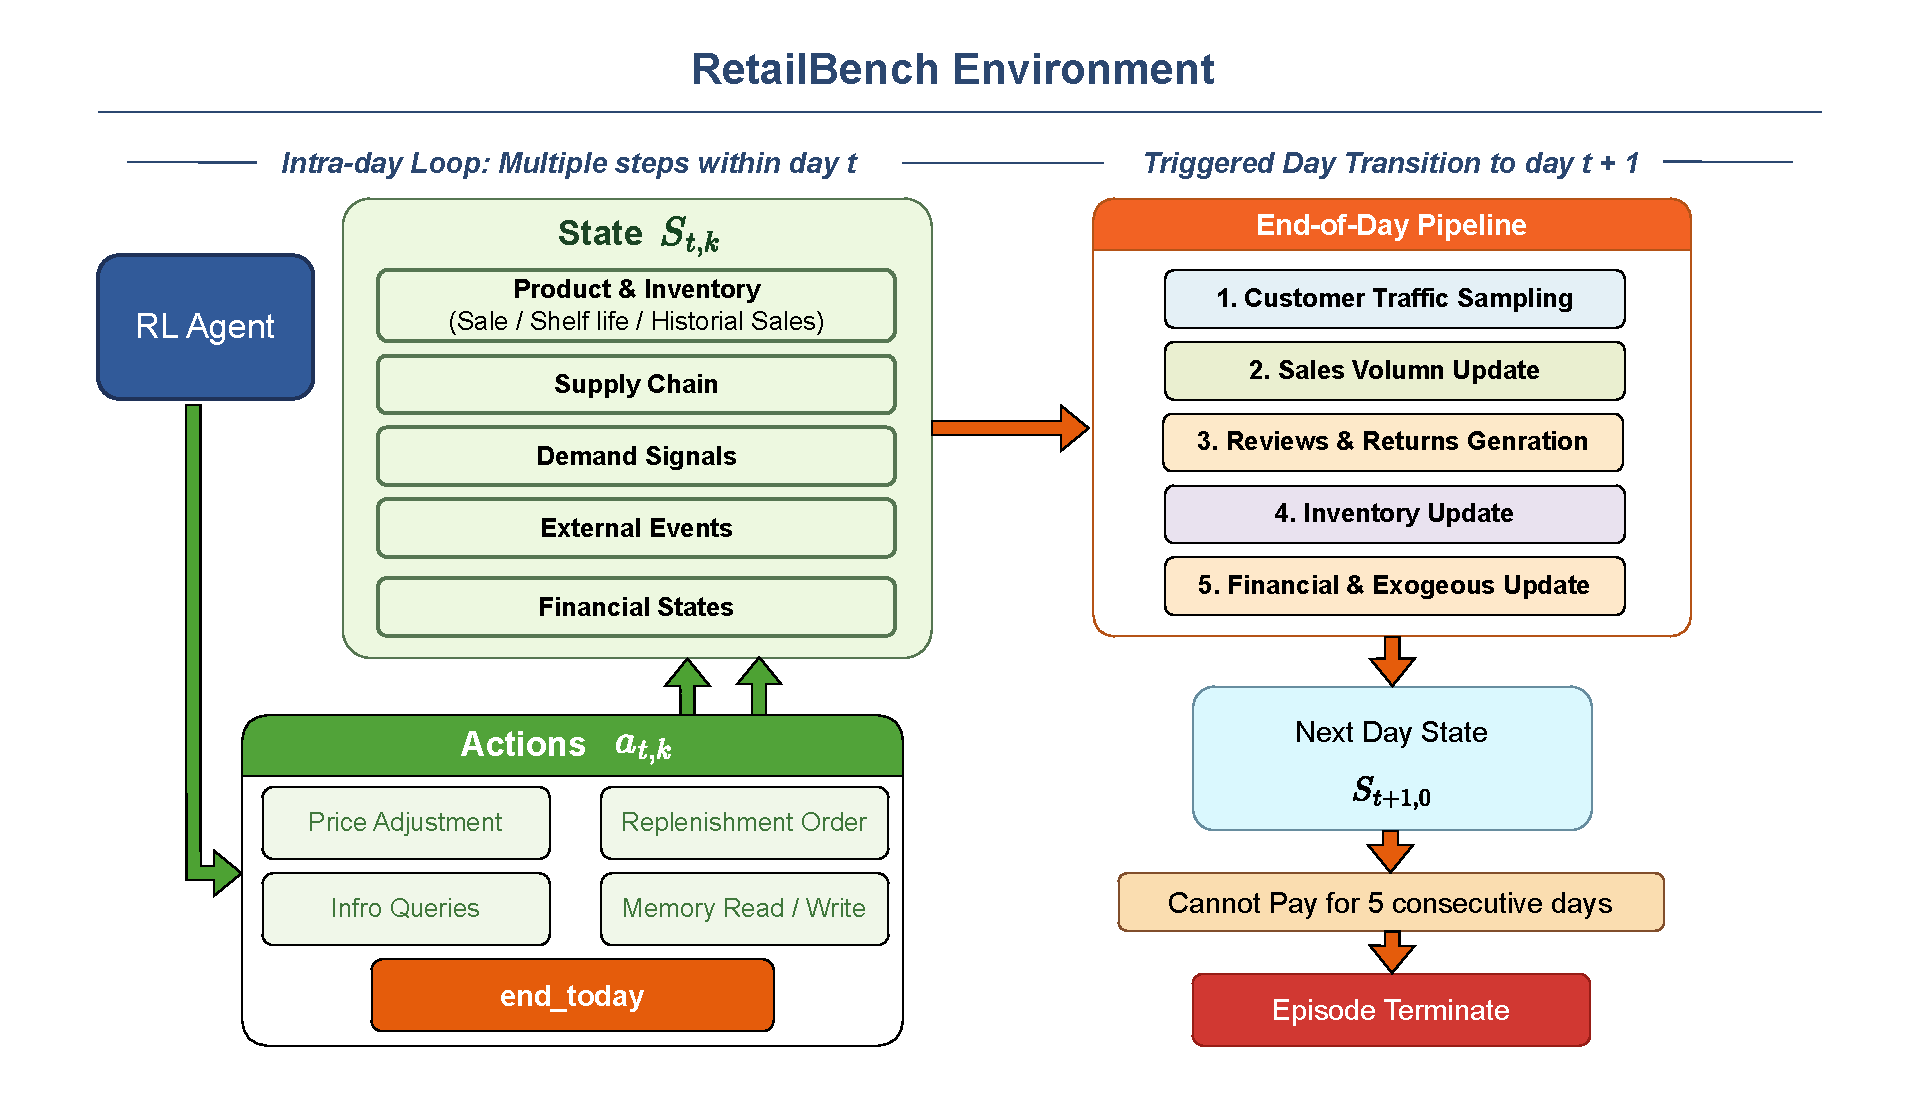
\includegraphics[width=\linewidth]{figures/env.pdf}
\end{center}
\caption{
Overview of the hierarchical supermarket environment, illustrating intra-day agent–environment interactions and end-of-day state transition dynamics.
}
\label{fig:workflow}
\vspace{-5mm}
\end{figure*}

To systematically study this challenge, we introduce \textit{RetailBench}, a benchmark that incorporates elements from retail operations and economic modeling principles. RetailBench centers on a supermarket operation scenario that demands long-horizon decision-making, sustained interaction with a dynamic environment, and the integration of heterogeneous historical information. The benchmark evaluates whether LLM-based agents can sustain business operations under stochastic, multi-factor conditions.


We evaluate eight state-of-the-art LLMs and find that current models struggle to maintain stable decisions as the decision space expands, often fail to incorporate relevant information, and frequently exhibit hallucinations and economically irrational behaviors that lead to environment collapse.

Our contributions are summarized as follows:
\begin{itemize}[leftmargin=*]
    \item We introduce \textit{RetailBench}, an open-source benchmark for evaluating long-horizon decision-making in simulated retail environments, characterized by coupled pricing-inventory control, stochastic demand, and multi-day planning horizons.
    \item Through experiments across eight models and three environment configurations, we identify and quantify four systematic failure patterns that prevent current LLM-based agents from sustaining long-horizon operations: (1) non-scalable decision-making, (2) incomplete information coverage, (3) temporal instability, and (4) invalid actions.
    \item We propose the \textit{Evolving Strategy \& Execution} framework as a reference implementation that separates high-level strategy formulation from low-level execution. In our experiments, this framework achieves improved operational stability compared to day-level Reflection baselines, though substantial gaps remain relative to heuristic policies.
\end{itemize}
